%%%%%%%%%%%%%%%%%%%%%%% file template.tex %%%%%%%%%%%%%%%%%%%%%%%%%
%
% This is a general template file for the LaTeX package SVJour3
% for Springer journals.          Springer Heidelberg 2010/09/16
%
% Copy it to a new file with a new name and use it as the basis
% for your article. Delete % signs as needed.
%
% This template includes a few options for different layouts and
% content for various journals. Please consult a previous issue of
% your journal as needed.
%
%%%%%%%%%%%%%%%%%%%%%%%%%%%%%%%%%%%%%%%%%%%%%%%%%%%%%%%%%%%%%%%%%%%
%
% First comes an example EPS file -- just ignore it and
% proceed on the \documentclass line
% your LaTeX will extract the file if required
\begin{filecontents*}{example.eps}
%!PS-Adobe-3.0 EPSF-3.0
%%BoundingBox: 19 19 221 221
%%CreationDate: Mon Sep 29 1997
%%Creator: programmed by hand (JK)
%%EndComments
gsave
newpath
  20 20 moveto
  20 220 lineto
  220 220 lineto
  220 20 lineto
closepath
2 setlinewidth
gsave
  .4 setgray fill
grestore
stroke
grestore
\end{filecontents*}
%
\RequirePackage{fix-cm}
%
%\documentclass{svjour3}                     % onecolumn (standard format)
%\documentclass[smallcondensed]{svjour3}     % onecolumn (ditto)
%\documentclass[smallextended]{svjour3}       % onecolumn (second format)
\documentclass[twocolumn]{svjour3}          % twocolumn
%
\smartqed  % flush right qed marks, e.g. at end of proof
%

%
\usepackage{mathptmx}      % use Times fonts if available on your TeX system
%
% insert here the call for the packages your document requires
%\usepackage{latexsym}
\usepackage[demo]{graphicx}
%\usepackage{graphicx}
\usepackage[caption = false]{subfig}
\graphicspath{ {./images/} }
\usepackage[round]{natbib}
\usepackage{amsmath}  
\usepackage{amsfonts} 
\usepackage{graphicx} 
\usepackage[usenames]{color}
\usepackage{mathtools}
\usepackage{algorithm}
\usepackage[noend]{algpseudocode}
\usepackage{float}
\usepackage[toc,title,page]{appendix}

\newcommand{\Real}{\mathbb R}
\newcommand{\E}{\mathbb{E}}
\newcommand{\s}{\mathbb{S}}
\renewcommand{\P}{\mathbb{P}}
\newcommand{\K}{\mathbb{K}}
\newcommand{\Q}{\mathbb{Q}}
\newcommand{\eps}{\varepsilon}
\newcommand{\diag}{\mathrm{diag}}
\newcommand{\nbr}{\mathrm{nbr}}
\newcommand{\F}{\mathcal{F}}
\newcommand{\Qm}{\mathcal{Q}}
\newcommand{\M}{\mathcal{M}}
\newcommand{\Z}{\mathcal{Z}}
\newcommand{\csimplex}{\bar{\mathcal{S}}^{d-1}}
\newcommand{\osimplex}{\mathcal{S}^{d-1}}
\newcommand{\LL}{\mathcal{L}}
\newcommand{\Hil}{\mathscr{H}}
\newcommand{\G}{\mathscr{G}}
\newcommand{\p}{\mathscr{P}}
\newcommand{\C}{\mathscr{C}}
\newcommand{\one}[1]{\mathbf{1}_{\{#1\}}}
\newcommand{\oneset}[1]{\mathbf{1}_{#1}}
\newcommand{\argmin}{\mathrm{argmin}}
\newcommand{\argmax}{\mathrm{argmax}}
\newcommand{\var}{\mathrm{Var}}
\newcommand{\cov}{\mathrm{Cov}}
\newcommand{\ind}{\mathrm{I}}
\newcommand{\D}{\mathrm{d}}
\newcommand{\Borel}{\mathscr{B}}
\newcommand{\ben}{\begin{enumerate}}
\newcommand{\een}{\end{enumerate}}
\newcommand{\ds}{\displaystyle}
\newcommand{\voila}{\hfill $\blacksquare$}
\newcommand{\Id}{\mathrm{Id}}
\renewcommand{\Re}{\mathrm{Re}}
\renewcommand{\vec}[1]{\mathbf{#1}}
\renewcommand{\d}[1]{\ensuremath{\operatorname{d}\!{#1}}}
\newcommand*\diff{\mathop{}\!\mathrm{d}}

\DeclareMathOperator{\esssupp}{ess\,supp}

\journalname{Statistics and Computing}

\begin{document} \sloppy
\bibliographystyle{plainnat}

\title{Sequential Importance Sampling With Corrections For Partially Observed States
%\thanks{Grants or other notes
%about the article that should go on the front page should be
%placed here. General acknowledgments should be placed at the end of the article.}
}

\author{Valentina Di Marco \and
        Jonathan Keith \and
        Daniel Spring}

\institute{Valentina Di Marco \at
              School of Mathematical Science, Monash University, Clayton Campus, VIC 3800, Australia \\
              Tel.: +61-4-23330509\\
              \email{valentina.dimarco@monash.edu}      
              \and
              Jonathan Keith \at
              School of Mathematical Science, Monash University, Clayton Campus, VIC 3800, Australia
              \and
              Daniel Spring \at
              School of Ecosystem and Forest Sciences, The University of Melbourne, Parkville, Victoria 3010, Australia}

\date{Received: date / Accepted: date}
% The correct dates will be entered by the editor

\maketitle

\begin{abstract}

We consider an evolving system for which a sequence of observations is being made, with each observation revealing additional information about current and past states of the system. We suppose each observation is made without error, but does not fully determine the state of the system at the time it is made. Our motivating example is drawn from invasive species biology, where it is common to know the precise location of invasive organisms that have been detected by a surveillance program, but at any time during the program there are invaders that have not been detected.

We propose a sequential importance sampling strategy to infer the state of the invasion under a Bayesian model of such a system. The strategy involves simulating multiple alternative states consistent with current knowledge of the system, as revealed by the observations. However, a difficult problem that arises is that observations made at a later time are invariably incompatible with previously simulated states.

To solve this problem, we propose a two-step iterative process in which states of the system are alternately simulated in accordance with past observations, then corrected in light of new observations. We identify criteria under which such corrections can be made while maintaining appropriate importance weights.

\keywords{ Sequential Importance Sampling \and Filtering \and Bayesian estimation \and Partially observed spaces \and Missing data}
% \PACS{PACS code1 \and PACS code2 \and more}
% \subclass{MSC code1 \and MSC code2 \and more}
\end{abstract}

\section{Introduction}
\label{sec:1}
This paper considers the problem of imputing missing data in the presence of incomplete observations made sequentially in time. We thus envisage data that consists of a series of correlated observations made sequentially, each of which is correct but only partially reveals the true state of the system. The main difficulty that arises in this context is that data missing at one time point can be revealed at a later time point, so that imputed missing values must later be corrected in light of new information.

Our original motivation for considering this problem was to facilitate analysis of {\color{blue} invasive species, where in an ongoing surveillance program the locations of invaders are regularly being detected. For detected invaders, the location can be precisely determined, but at any given time there is an unknown number of undetected organisms}, each with an unknown location. To infer the current extent of the invasion, we aim to impute plausible locations of undetected individuals, but these imputations are only informed guesses, and will require constant correction as new detections come to light.

In addition, new nests are constantly being produced: the unseen state of the system is thus constantly evolving. Knowing the location of at least some of the invaders at time $t$, we can simulate the evolution of this system. However, again the imputed locations of simulated nests will require constant correction as more information about the true state of the system becomes available.

Here we propose a new approach to problems of this type. Although our approach is ultimately aimed at inference for invasive species, we will illustrate the method for less complex evolving systems in which correct but partial observations are being made in real time.

To handle problems of this kind, we introduce a Bayesian approach that uses a new sequential importance sampling (SIS) strategy. As is typical of SIS methods, we generate a population of particles, each representing a plausible sequence of system states, and we evolve each particle at each time step according to a model of system dynamics. Again in a manner typical of SIS methods, new observations arrive in real time, and we use these observations to adjust the weights assigned to particles. However, a crucial new element in our method is that we allow missing values imputed at earlier time steps to be corrected so that they are consistent with the new observations.

Our method thus addresses a problem that is common in practice: new observations made in real time can render previously imputed missing values implausible, and may even conflict with what has been simulated. For example, in the invasive species context described above, undetected {\color{blue} invaders} imputed to geographic areas that do not contain any {\color{blue}invaders} become increasingly implausible as time passes without detections being made in those regions. In standard SIS approaches, such particles receive low weights and are eventually eliminated by resampling, but a common problem is that all particles can become implausible, if not inconsistent, with observations.

Problems of this kind arise in many contexts. We can envisage the approach being used to study the evolution of a species' geographic range, for both invasive and non-invasive species. The algorithm could also be applied to a variety of other missing data problems where new incomplete data is continuously acquired, such as in crime prediction, (\cite{Malathy}) or bushfire modeling (\cite{Beer}). Another potential application is in the study of the spread of infectious diseases, where observations are made in the form of diagnosed cases, but there is missing data in the form of undiagnosed cases (\cite{O'Neill}). 

Missing data are ubiquitous in ecological and evolutionary data sets as in many other branches of science. Two common methods used to deal with missing data are to delete rows of a data matrix (corresponding to individuals or cases) that are missing data, or to use the mean to fill in missing values. However, these methods result in biased estimation of parameters and uncertainty, and reduction in statistical power. Better missing data procedures such as data augmentation (\cite{Tanner}) and multiple imputation (\cite{RubinMI}) are available  (\cite{Nakagawa}).
{\color{blue} For an up-to-date treatment of missing data in statistics see \cite{Little}}.

{\color{blue}Techniques like multiple imputations and data augmentation, in general do not use past observations and the state transition equations when estimating the probability of the hidden state knowing the observations. This can result in poor performance when the problem can be well modelled, for example, by a Markov structure (\cite{Zhang}).}

{\color{blue} An example of a methodology for dealing with missing data in the context of a Markov structure} is the Multiple Imputation Particle Filter (MIPF) developed by \cite{Zhang}. This method, {\color{blue}applied to signal processing}, uses randomly drawn values (imputations) to provide a replacement for the missing data and then uses the particle filter to estimate non-linear state with the data, where a {\color{blue} Non-linear state estimations deals with estimation of input states, provided a measurement sequence from a sensor with the unknown input sequence.}

Particle filters are sometimes used to estimate a hidden state when partial, noisy observations are made. However, the performance of particle filtering algorithms can severely degrade in the presence of missing data (\cite{Zhang}).

{\color{blue} For a comprehensive discussion of the applications of particle filters, also called Sequential Monte Carlo (SMC) methods see \cite{Cappe} and \cite{Doucet}.}

{\color{blue} In particular sequential importance sampling, in the form of sequential imputation firstly introduced by \cite{Kong}, have been used in Bayesian missing data problems in situations where the posterior must be constantly updated with the arrival of new data.}

Here we propose a two-step iterative procedure for dynamically updating a collection of weighted particles used to represent a posterior distribution over the possible trajectories of a partially observed system. In the first step, we evolve particles in accordance with a model of the system, in a manner common to particle-based sequential Monte Carlo methods. In the second step, we correct the particles in light of newly acquired data. The method treats an uncorrected particle (generated in the first step) as a form of augmented variable. Thus the method constitutes a novel use of augmentation in sequential importance sampling. 

Our method deals with situations where the data are informative, a situation where standard sequential Monte Carlo methods can perform poorly {\color{blue}\cite{Del Moral}}. {\color{red} (HHH I don't understand what you mean by `informative' in that sentence. I think all statistical methods require data that is informative.)}
{\color{blue}HHH With informative observations I mean when there is very little noise present for the observation process relative to the amount of process noise. In this case standard SMC methods perform poorly as mentioned by Del Moral, but perhaps this is true only when the process is observed indirectly? Our case though, is a special case of indirect observations with $p(z_n | x_n) = \delta (z_n - x_n)$, where $z_n$ are the observations and $x_n$ the hidden states. so I though it was worth mentioning that SMC in general don't perform well with precise observations. This is my understanding: let us consider a hidden state model $x$ and observation values $z$ with very little noise (informative). 
\begin{equation}
    x_t | x_{1:t-1} \sim f(x_t | x_{t-1})
\end{equation}
\begin{equation}
    z_t = g(x_t)
\end{equation}
with $g$ a deterministic mapping. Let us consider a standard boostrap filter to provide estimates, for example, of the likelihood $p(z_{1:n} | \theta)$ where $\theta$ are the parameters. In the filter we will draw $N$ particles $\{ y^i_n\}_{i=1:N}$ from equation 1 then we calculate the weights multiplying the weights for the previous time with the values from equation 2. As long as there is at least one particle $y^j_n$ which gives a reasonably high probability for the measurement $z_t$ (and consequently gets assigned a large weight), the particle filter will provide a reasonable result, and the more such high-weight particles, the better (in terms of variance of the estimate $\hat{p}(z_{1:n} | \theta)$). However, if no samples $y_n$ are drawn under which $z_t$ could have been observed with reasonably high probability, the estimate will be poor. If there is very little measurement noise but non-negligible process noise in the model, the chance of drawing any useful particles by simulating the system dynamics would be small. Am I correct in saying so?}

\cite{Del Moral} proposed a Sequential Monte Carlo method for sampling the posterior distribution of state-space models under highly informative observation regimes. In their method they introduce a schedule of intermediate weighting and resampling times between observation times, which guides particles towards the final state.

\cite{Finke} developed a Particle Monte Carlo Markov Chain algorithm to estimate the demographic parameters of a population and then incorporated this algorithm into a sequential Monte Carlo sampler in order to perform model comparison motivated by the fact that a simple importance sampling performs poorly if there is a strong mismatch between the prior and the posterior, which is common when the data is highly informative. {\color{blue}HHH I am not sure we need to mention Finke if we don't want to put focus on highly informative observations.}

In this paper, we provide a proof of concept for our proposed methodology using a simple system modelled by an AR(1) process and a model for an invasive species in a river. In these examples, we present a version of our method in which only those imputed values that are strictly inconsistent with later observations are corrected in a deterministic manner. 
In Section 1 we describe the new method. In Section 2 we apply the method to a simple stationary AR(1) model and compare our results with an analytic approach for the estimation of missing elements in stationary AR(1) models.
In Section 3 we apply the method to a river invasion and illustrate how it can be used to infer the extent of the invasion.
The last chapter contains our conclusions and proposes future directions for research.

\section{Sequential Importance Sampling with corrections}
\label{sec:2}

Consider an $M$-dimensional system, evolving in discrete time. The states of this system at times $t = 1, \dots, T$ are represented by random vectors $\vec{x}^t = (x^t_1, \dots, x^t_M) \in \Real^M$ defined on a probability space $(\Omega, \F, \P)$. The trajectory of the system up to time $t$ we represent by a random matrix $\vec{X}^t = (\vec{x}^1, \ldots, \vec{x}^t)$. We also represent our state of knowledge regarding the trajectory of the system up to time $t$ by a random binary matrix $\vec{B}^t = (b^t_{im}) \in 2^{T \times M}$, where $b^t_{im} = 1$ if the value of $x^i_m$ is known by time $t$, and $b^t_{im} = 0$ if the value of $x^i_m$ is still unknown at time $t$. Note that once a past system coordinate $x^i_m$ is known, it cannot become unknown, so $b^t_{im} = 1$ implies $b^{t^\prime}_{im} = 1$ at all later times $t^{\prime} > t$, and similarly $b^t_{im} = 0$ implies $b^{t^{\prime}}_{im} = 0$ at all earlier times $t^{\prime} < t$. {\color{red} Jon, why do we define $\vec{B}^t = (b^t_{im}) \in 2^{T \times M}$ and not $\vec{B}^t = (b^t_{im}) \in 2^{t \times M}$ or $\vec{B}^T = (b^T_{im}) \in 2^{T \times M}$? (The same for the function $\sigma$ below, shouldn't it be $\sigma: \Real^{t \times M} \times 2^{t \times M} \rightarrow (\Real \cup \{ - \})^{t \times M}$?)} {\color{blue} Feel free to define them in the way you propose. I think both are valid, and I have no preference.}

It will also be useful to define an {\em observation matrix} $\vec{Z}^t = (z^t_{im})$, where $z^t_{im} = x^i_m$ if $b^t_{im} = 1$, and $z^t_{im} = -$ if $b^t_{im} = 0$. Thus the symbol `$-$' is used to represent an unknown system coordinate. We assume that observations are made without error, so that $\vec{Z}^t$ is fully determined by $\vec{X}^t$ and $\vec{B}^t$. We therefore define a function $\sigma: \Real^{T \times M} \times 2^{T \times M} \rightarrow (\Real \cup \{ - \})^{T \times M}$ such that $\vec{Z}^t = \sigma(\vec{X}^t, \vec{B}^t)$.

For each past system coordinate $x^i_m$ that has not been observed by time $t$ (so that $b^t_{im} = 0$) there may nevertheless be some information that can be derived from the observations and a model of the system. We take a Bayesian approach to quantify this information. At time $t=1$, our knowledge of the system is represented by a prior distribution with density $q(\vec{X}^1, \vec{B}^1)$ on $\Real^M \times 2^M$ and the posterior distribution after observing $\vec{Z}^1$ has a density on $\sigma^{-1}(\vec{Z}^1)$ given by:
\begin{equation*}
    p(\vec{X}^1, \vec{B}^1 |\vec{Z}^1) =
        \frac{q(\vec{X}^1, \vec{B}^1)}
        {r(\vec{Z}^1)} 
\end{equation*}
where
\begin{align*}
    r(\vec{Z}^1)  &= \int q(\vec{X}^1, \vec{B}^1) \prod_{ \{m \in \{1, \ldots, M \} : z^1_{1m} = - \} } \D x^1_m.
\end{align*}
Note that $\vec{B}^1$ is fully determined by $\vec{Z}^1$, since $b^1_{1m} = 0$ wherever $z^1_{1m} = -$ and $b^1_{1m} = 1$ otherwise.

Our knowledge of the trajectory of the system at time $t \geq 2$, before we acquire the next observation matrix $\vec{Z}^t$, is represented by a prior distribution with density $q(\vec{X}^t, \vec{B}^t | \vec{Z}^{t-1})$ on the subspace $\sigma^{-1}(\vec{Z}^{t-1}) \times \Real^M \times 2^M \subseteq \Real^{tM} \times 2^{tM}$. {\color{red} Jon, I don't think I understand this, I thought this would have to be $\sigma^{-1}(\vec{Z}^{t-1}) \times \Real^{M} \times 2^{M} \subseteq \Real^{t \times M} \times 2^{t \times M}$ as we have used this notation before, what do we mean with $\Real^{tM}$ and $2^{tM}$?} {\color{blue} I mean $t \times M$, so use that if you prefer, I just thought $tM$ was more concise.} After observing $\vec{Z}^t$, certain pairs $(\vec{X}^t, \vec{B}^t)$ with non-zero prior density will be incompatible with the new observations, and the posterior density must therefore restrict $(\vec{X}^t, \vec{B}^t)$ to $\sigma^{-1}(\vec{Z}^t)$. The posterior density over $\sigma^{-1}(\vec{Z}^t)$ must therefore be
\begin{equation*}
    p(\vec{X}^t, \vec{B}^t |\vec{Z}^t) =
        \frac{q(\vec{X}^t, \vec{B}^t | \vec{Z}^{t-1})}
        {r(\vec{Z}^t | \vec{Z}^{t-1})} 
\end{equation*}
where $q$ is restricted to $\sigma^{-1}(\vec{Z}^t)$ and
\begin{align*}
    r(\vec{Z}^t | \vec{Z}^{t-1})  &= \int q(\vec{X}^t, \vec{B}^t | \vec{Z}^{t-1}) \prod_{ \{ i \leq t, m \in \{1, \ldots, M \} : z^t_{im} = - \} } \D x^i_m.
\end{align*}
Note that $\vec{Z}^t$ fully determines $\vec{B}^t$ and those elements $x_m^i$ of $\vec{X}^t$ for which $b_{im}^t = 1$, and that the preceding equation integrates over the remaining elements of $\vec{X}^t$. Thus $r(\vec{Z}^t | \vec{Z}^{t-1})$ is effectively the integral of $q(\vec{X}^t, \vec{B}^t | \vec{Z}^{t-1})$ over $\sigma^{-1}(\vec{Z}^t)$, where $\vec{Z}^{t} = \sigma(\vec{X}^t, \vec{B}^t)$. We will abuse notation slightly by reinterpreting $\sigma^{-1}(\vec{Z}^t)$ as a subset of $\Real^{tM}$, since the second co-ordinate $\vec{B}^t$ is the same for all $(\vec{X}^t, \vec{B}^t) \in \sigma^{-1}(\vec{Z}^t)$. 

In this paper we focus on Markovian systems, that is, systems in which each $\vec{x}^t$ is conditionally independent of $\vec{X}^{t-2} = (\vec{x}^1, \ldots,\vec{x}^{t-2})$, given $\vec{x}^{t-1}$. Let $f(\vec{x}^t | \vec{x}^{t-1})$ be the transitional density distribution characterising the system. We also suppose that our current state of knowledge regarding the trajectory of the system up to and including the current time depends on both the trajectory of the system and our knowledge of it at the previous time, as follows:
\begin{align*}
    &\vec{x}^t | \vec{x}^{t-1} \sim f(\vec{x}^t | \vec{x}^{t-1})\\
    &\vec{B}^t | \vec{X}^t, \vec{B}^{t-1} \sim g(\vec{B}^t | \vec{X}^t, \vec{B}^{t-1})
\end{align*}
for $t \geq 2$, with densities of the initial states $f(\vec{x}^1)$ and $g(\vec{B}^1 | \vec{x}^1)$. This general framework allows for the possibility that $\vec{B}^t$ is independent of $\vec{X}^{t}$ and depends only on $\vec{B}^{t-1}$. It also allows for the alternative possibilities that observations are made in response to what is known about the trajectory of the system and/or that the probability of making an observation depends on the trajectory of the system. Thus the joint prior distribution for $(\vec{X}^t,\vec{B}^t)$ when $t=1$ is given by 
\[
q(\vec{X}^1,\vec{B}^1) = f(\vec{x}^1)g(\vec{B}^1 | \vec{x}^1)
\]
and when $t \geq 2$: 
\begin{eqnarray*}
    q(\vec{X}^t, \vec{B}^t | \vec{Z}^{t-1}) &=& f(\vec{x}^t | \vec{x}^{t-1}) g(\vec{B}^t | \vec{X}^t, \vec{B}^{t-1}) p(\vec{X}^{t-1}, \vec{B}^{t-1} | \vec{Z}^{t-1}) \\
& = & \frac{f(\vec{x}^1)g(\vec{B}^1 | \vec{x}^1)}{r(\vec{Z}^1)} \prod_{i=2}^{t-1} \frac{f(\vec{x}^i | \vec{x}^{i-1}) g(\vec{B}^i | \vec{X}^i, \vec{B}^{i-1})}{r(\vec{Z}^i | \vec{Z}^{i-1})} \\
& & \times f(\vec{x}^t | \vec{x}^{t-1}) g(\vec{B}^t | \vec{X}^t, \vec{B}^{t-1})
\end{eqnarray*}
on $\sigma^{-1}(\vec{Z}^{t-1}) \times \Real^M \times 2^M$, and the joint posterior distribution is given by:
\begin{eqnarray*}
    p(\vec{X}^t, \vec{B}^t | \vec{Z}^t) 
& = & \frac{f(\vec{x}^1)g(\vec{B}^1 | \vec{x}^1)}{r(\vec{Z}^1)} \prod_{i=2}^t \frac{f(\vec{x}^i | \vec{x}^{i-1}) g(\vec{B}^i | \vec{X}^i , \vec{B}^{i-1})}{r(\vec{Z}^t | \vec{Z}^{t-1})} 
\end{eqnarray*}
on $\sigma^{-1}(\vec{Z}^t)$. For the purpose of calculation, it is helpful to define
\begin{eqnarray*}
r(\vec{Z}^1,\ldots,\vec{Z}^t) & := & r(\vec{Z}^1) \prod_{i=2}^{t} r(\vec{Z}^i | \vec{Z}^{i-1}) \\
& = & \int  h(\vec{X}^t,\vec{B}^1,\ldots,\vec{B}^t) \prod_{ \{ i \leq t, m \in \{1, \ldots, M \} : z^t_{im} = - \} } \D x^i_m.
\end{eqnarray*}
where
\begin{eqnarray*}
h(\vec{X}^t,\vec{B}^1,\ldots,\vec{B}^t) & := & f(\vec{x}^1)g(\vec{B}^1 | \vec{x}^1) \prod_{i=2}^{t} f(\vec{x}^i | \vec{x}^{i-1}) g(\vec{B}^i | \vec{X}^i , \vec{B}^{i-1}).
\end{eqnarray*}

If $\vec{B}^t$ evolves independently of $\vec{X}^t$, the $g$ terms can be brought outside the integrals in the expressions above. Thus all $g$ terms cancel in the above expression for $p(\vec{X}^t, \vec{B}^t | \vec{Z}^t)$. Moreover, all $g$ terms except the final term $g(\vec{B}^t | \vec{B}^{t-1})$ cancel in the above expression for $q(\vec{X}^t, \vec{B}^t | \vec{Z}^{t-1})$ and this last term may be removed by summing over $\vec{B}^t$. In this case, it will be convenient to define
\begin{eqnarray*}
h(\vec{X}^t) & := & f(\vec{x}^1)\prod_{i=2}^{t} f(\vec{x}^i | \vec{x}^{i-1})
\end{eqnarray*}
and
\begin{eqnarray*}
r(\vec{Z}^t) & := & \int  h(\vec{X}^t) \prod_{ \{ i \leq t, m \in \{1, \ldots, M \} : z^t_{im} = - \} } \D x^i_m
\end{eqnarray*}
and to redefine
\begin{eqnarray*}
r(\vec{Z}^t | \vec{Z}^{t-1}) & := & \frac{r(\vec{Z}^t)}{r(\vec{Z}^{t-1})}.
\end{eqnarray*}
With this modified notation, we can now write:
\[
q(\vec{X}^1) = f(\vec{x}^1),
\]
and for $t \geq 2$,
\begin{eqnarray*}
    q(\vec{X}^t | \vec{Z}^{t-1}) & = & \frac{f(\vec{x}^1)}{r(\vec{Z}^1)}  \prod_{i=2}^{t-1} \frac{f(\vec{x}^i | \vec{x}^{i-1}) }{r(\vec{Z}^t | \vec{Z}^{t-1})} f(\vec{x}^t | \vec{x}^{t-1})
\end{eqnarray*}
on $\sigma^{-1}(\vec{Z}^{t-1}) \times \Real^M $ and 
\begin{eqnarray*}
    p(\vec{X}^t | \vec{Z}^t) 
& = & \frac{f(\vec{x}^1)}{r(\vec{Z}^1)} \prod_{i=2}^t \frac{f(\vec{x}^i | \vec{x}^{i-1}) }{r(\vec{Z}^t | \vec{Z}^{t-1})} 
\end{eqnarray*}
on $\sigma^{-1}(\vec{Z}^t)$.







We want to approximate the distribution $p(\vec{X}^{t}, \vec{B}^{t} | \vec{Z}^{t})$ by iterative sampling, and thus obtain Monte Carlo estimates of expectations of the form:
\begin{equation*}
    E_{p} \Big[l(\vec{X}^{t}, \vec{B}^{t} ) \Big] = \int l(\vec{X}^{t}, \vec{B}^{t})\; p(\vec{X}^{t}, \vec{B}^{t} | \vec{Z}^{t})\; \D \vec{X}^{t}
\end{equation*}
for functions {\color{red}$l: \Real^{t \times M} \times 2^{t \times M} \rightarrow \Real$}. 

We take a sequential importance sampling approach, at each iteration using a collection of weighted particles to represent $p(\vec{X}^{t-1}, \vec{B}^{t-1} | \vec{Z}^{t-1})$ from the previous iteration, in the sense that these particles can be used to construct weighted Monte Carlo estimates for integrals of the above form. We evolve these under the model to create a new set of weighted particles representing the prior for iteration $t$, namely $q(\vec{X}^{t}, \vec{B}^{t} | \vec{Z}^{t-1})$. We then modify these particles to be consistent with the observations $\vec{Z}^{t}$, and adjust the weights to ensure the resulting weighted particles represent our posterior $p(\vec{X}^{t}, \vec{B}^{t} | \vec{Z}^{t})$.

Consider a particle $(\vec{X}^{t-1},\vec{B}^{t-1})$ constructed at time point $t$, one of $n$ such particles. {\color{red} (HHH Consider adding a particle index as a subscript.)} We generate $\vec{x}^t$ for this particle by sampling from $f(\vec{x}^t | \vec{x}^{t-1})$. Similarly, we generate $\vec{b}^{t}$ for this particle by sampling from $g(\vec{b}^{t} | \vec{x}^t, \vec{b}^{t-1})$. However, the new vector of observations $\vec{z}^{t}$ is typically inconsistent with a particle $(\vec{X}^{t}, \vec{B}^{t})$ thus constructed, in two ways: first, the coordinates at which $\vec{b}^{t}$ contains a 0 may not correspond to the coordinates at which $\vec{z}^{t}$ contains a `$-$' {\color{red} shouldn't we mention also that coordinates at which $\vec{b}^{t}$ contains a newly generated 1 may not correspond to an observation in $\vec{z}^{t}$?}, and second, the observed values in $\vec{z}^{t}$ differ from the corresponding coordinates of $\vec{x}^{t}$. We must therefore correct $\vec{x}^{t}$ and $\vec{b}^{t}$ in light of the new observations $\vec{z}^{t}$. The simplest way to do this is to first replace $\vec{b}^{t}$ with the unique binary vector $\vec{(b')}^{t}$ that is consistent with $\vec{z}^{t}$, and then replace the coordinates of $\vec{x}^{t}$ with the corresponding coordinates of $\vec{z}^{t}$ wherever $\vec{(b')}^{t}$ has a `1', thus generating a corrected term $\vec{(x')}^{t}$. The corrections thus made at time point $t$ will be carried forward into the particles used at all future times. Note that we are considering the corrections to be deterministic, that is, $\vec{(x')}^{t}$ and $\vec{(b')}^{t}$ are deterministic functions of $\vec{x}^{t}$ and $\vec{b}^{t}$.

At each iteration, in order to simulate via a two-step process in which we generate a sample and then correct in light of data, we propose to introduce an auxiliary variable into importance sampling. The auxiliary variable will be the yet to be corrected sample $(\vec{X}^{t}, \vec{B}^{t})$ at time $t$ {\color{red} which is an element of the space $\Omega = \sigma(\vec{Z}^{t-1}) \times \mathbb{R}^M \times 2^M$}. Since the corrections are deterministic, the simulated pair {\color{red}$(\vec{X}^t, \vec{B}^t)$ can only be corrected in one way $(\vec{(X')}^t, \vec{(B')}^t) \in \sigma^-1(\vec{z}^t)$. We will use a projection map $\pi$ to relate the augmented space $\Omega^* = \Omega \times \sigma^{-1}(\vec{z}^t)$ containing the elements $(\vec{(X')}^{t}, \vec{(B')}^{t}, \vec{X}^{t}, \vec{B}^{t})$ to the corrected state space $\sigma^{-1}(\vec{z}^t)$ containing $(\vec{(X')}^{t}, \vec{(B')}^{t})$. Then, we apply importance sampling to be able to estimate the expectation $E_{p}[l(\vec{(X')}^{t},\vec{(B')}^{t})]$ sampling from the known distribution $q$.}

For simplicity, let us call $(\vec{X}^{t}, \vec{B}^{t}) = \vec{y}^{t}$ and $(\vec{(X')}^{t}, \vec{(B')}^{t}) = \vec{(y')}^{t}$.

Our strategy is to define a probability $\P^*$ having density $p^*$ on $\Omega^*$ such that the marginal distribution of $\P^*$ on {\color{red} $\sigma^{-1}(\vec{z}^t)$} is $\P$, that is $\P = \P^* \circ \pi^{-1}$. By the the disintegration theorem (see \cite{Rohlin}) it follows that there exist a family of {\color{red}Lebesgue} measures $\{ \nu_{\vec{(y')}^t} \}_{\vec{(y')}^t \in \Omega'}$ on $\Omega^*$ such that for every measurable Borel function $m:\Omega^* \rightarrow [0, \infty]$
\begin{align*}
    &\int_{\Omega^*} m(\vec{(y')}^t, \vec{y}^t)\diff (\vec{(y')}^t,\vec{y}^t) = \\
    & \int_{{\color{red}\sigma^{-1}(\vec{z}^t)}} {\color{red} \bigg( }\int_{\pi^{-1}(\vec{(y')}^t)} m(\vec{(y')}^t, \vec{y}^t) (\diff \vec{(y')}^t {\color{red} | } \vec{y}^t) {\color{red} \bigg) } \diff \vec{\vec{y'}}.
\end{align*}
{\color{red} Jon, would it make it easier to understand if we introduced the measures back into the integrals?} 
It follows that for any event $A \in \F'$ where $\F'$ is the $\sigma$-algebra over {\color{red}$\sigma^{-1}(\vec{z}^t)$},
\begin{align*}
    &\P(A) = \P^{\color{red}*}(\pi^{-1}(A)) = \\
    &\int_{\Omega^*} I_A(\pi(\vec{(y')}^t, \vec{y}^t)) p^*(\vec{(y')}^t, \vec{y}^t | \vec{Z}^t) \D (\vec{(y')}^t, \vec{y}^t) = \\
    & \int_{{\color{red}\sigma^{-1}(\vec{z}^t)}} I_A(\vec{(y')}^t \Bigg[ \int_{\pi^{-1}(\vec{(y')}^t)} p^*(\vec{(y')}^t, \vec{y}^t | \vec{Z}^t) \D {\color{red}  \vec{y}^t}  \Bigg] \D \vec{(y')}^t
\end{align*}
and hence
\begin{equation*}
    p(\vec{(y')}^t | \vec{Z}^t) = \int_{\pi^{-1}((\vec{y}')^t)} p^*(\vec{(y')}^t, \vec{y}^t | \vec{Z}^t)\; \D {\color{red} \vec{y}^t}.
\end{equation*}
Moreover,
\begin{align*}
    &E_{p}[l(\vec{(y')}^{t})]  = \int_{{\color{red}\sigma^{-1}(\vec{z}^t)}} l(\vec{(y')}^{t})\; p(\vec{(y')}^{t} | \vec{Z}^{t}) \D \vec{(y')}^{t} \\
    &= \int_{{\color{red}\sigma^{-1}(\vec{z}^t)}} l(\vec{(y')}^{t})\Bigg[\int_{\pi^{-1}(\vec(y'))} p^*(\vec{(y')}^{t}, \vec{y}^{t} | \vec{Z}^{t}) \D {\color{red} \vec{y}^t} \Bigg] \D \vec{(y')}^{t} \\ 
    &= \int_{\Omega^*} l(\pi(\vec{(y')}^{t}, \vec{y}^{t}))\; p^*(\vec{(y')}^{t}, \vec{y}^{t} | \vec{Z}^{t}) \D (\vec{(y')}^t, \vec{y}^t) \\ 
    &= E_{p^*}[l(\pi (\vec{(y')}^{t}, \vec{y}^{t}))].
\end{align*}
Applying importance sampling on the probability space $\Omega^*$ with the probability measures $\P$ and $\Q$ with densities $p$ and $q$ respectively where $\q$ is the known distribution, we get
\begin{align*}
    E_{p^*}[l(\pi (\vec{(y')}^{t}, \vec{y}^{t})] = \int_{\Omega^*} l(\pi(\vec{(y')}^{t}, \vec{y}^{t})) \frac{p^*(\vec{(y')}^{t}, \vec{y}^{t}|\vec{Z}^{t})} {q(\vec{(y')}^{t}, \vec{y}^{t} | \vec{Z}^{t-1})} \\
    q(\vec{(y')}^{t}, \vec{y}^{t} | \vec{Z}^{t-1}) \; \D \vec{y}^{t} \approx \sum_{i=1}^n  w^{t}_i l(\pi (\vec{(y')}^{t}_i, \vec{y}^{t}_i))
\end{align*}
where the weights $w^{t}_i$ are:
\begin{equation*}
    w^{t}_i = \frac{p^*(\vec{(y')}^{t}_i, \vec{y}^{t}_i | \vec{Z}^{t})} {p(\vec{(y')}^{t}_i, \vec{y}^{t}_i|\vec{Z}^{t-1})}.
\end{equation*}
In our examples with deterministic substitutions $p^*$ will simply be:
\begin{equation*}
    p^*(\vec{(y')}^{t}, \vec{y}^{t} | \vec{Z}^{t}) = p(\vec{(y')}^{t} | \vec{Z}^{t}) = \frac{ q(\vec{(y')}^{t}|\vec{Z}^{t-1})} {r(\vec{Z}^{t} | \vec{Z}^{t-1})}
\end{equation*}
and
\begin{equation*}
    q(\vec{(y')}^{t}, \vec{y}^{t} | \vec{Z}^{t-1}) = q(\vec{y}^{t} | \vec{Z}^{t-1})
\end{equation*}
therefore the normalised weights $w^t$ will be:

\begin{multline*}
    w^{t} = \frac{q(\vec{(y')}^{t}_i | \vec{Z}^{t-1}) }{q(\vec{y}^{t}_i | \vec{Z}^{t-1})}\Bigg( \sum_{i=1}^n  \frac{q(\vec{(y')}^{t}_i | \vec{Z}^{t-1}) }{q(\vec{y}^{t}_i | \vec{Z}^{t-1})}\Bigg)^{-1} = \\
    \frac{q(\vec{({\color{red}X}')}^{t}_i, \vec{(B')}^{t}_i | \vec{Z}^{t-1}) }{q(\vec{{\color{red}X}}^{t}_i, \vec{B}^{t}_i | \vec{Z}^{t-1})}\Bigg( \sum_{i=1}^n \frac{q(\vec{({\color{red}X}')}^{t}_i, \vec{(B')}^{t}_i | \vec{Z}^{t-1}) }{q(\vec{{\color{red}X}}^{t}_i, \vec{B}^{t}_i | \vec{Z}^{t-1})}\Bigg)^{-1}
\end{multline*}
since the constant $r(\vec{Z}^t | \vec{Z}^{t-1})$ of $q(\vec{{\color{red}X}}^{t-1}_i,\vec{B}^{t-1}_i | \vec{Z}^{t-1})$ cancels out after normalisation.

In order to be able to apply importance sampling we will need to prove that $\esssupp(p^*) \subseteq \esssupp(q)$
which is obvious when we consider deterministic substitutions where $p^*(\vec{(y')}^{t}, \vec{y}^{t} | \vec{Z}^{t}) \propto q(\vec{(y')}^{t}|\vec{Z}^{t-1})$.

\section{Application to a stationary AR(1) model}
\label{sec:3}

Let us first introduce our importance sampling idea using a simple example. Consider a linear, normal and stationary AR(1) process for which
\begin{equation*}
    x_{t} = \varphi x_{t-1} + \eps_{t}
\end{equation*}
with $\eps_{t} \stackrel{iid}{\sim} \mathcal{N}(0, \sigma^{2})$. Then
\begin{equation*}
    (x_{t} | x_{t-1}) \sim \mathcal{N} (\varphi x_{t-1}, \sigma^{2}).
\end{equation*}
This process is stationary provided that the initial distribution is
\begin{equation*}
    x_{1} \sim \mathcal{N} \Bigg (0, \frac{\sigma^2}{1- \varphi^2} \Bigg )
\end{equation*}
which is valid only if $|\varphi| < 1$.

Suppose that at any time $t$, only some subset of the values $\vec {x}^{t} = (x_1, \dots, x_{t})$ have so far been observed. However, those that have been observed are known without error. We collect the values that have been observed at or before time $t$ to form a vector $\vec{z}^{t} = (z_1^{t}, \dots, z_{t}^{t})$, where for each $s \leq t$, $z_s^{t} = x_s$ if $x_s$ has been observed at or before time $t$ and $z_s^{t} = -$ otherwise. Thus the coordinates of $\vec{z}^{t}$ belong to an extension of the reals $\mathbb{R} \cup \{ - \}$.

As time progresses, new observations become available. Thus some dashes in the vector $\vec{z}^{t}$ will be replaced by observations in the subsequent vector $\vec{z}^{t+1}$. However, the reverse does not occur: if we have $z_s^{t} = x_s$ for times $s$ and $t$ where $s \leq t$ then we must also have $z_s^{t^{\prime}} = x_s$ at all subsequent times $t^{\prime} > t$.

We will therefore define a lower triangular $t \times t$ matrix $\vec{Z}^{t}$ in which row $i$ is the vector $\vec{z}^{i}$.

We will also define binary vectors $\vec{b}^{t} = (b_1^{t}, \dots, b_{t}^{t})$, where $b_s^{t} = 1$ if $z_s^{t} = x_s$, and $b_s^{t} = 0$ if $z_s^{t} = -$, and a lower triangular $t \times t$ binary matrix $\vec{B}^{t}$ in which row $i$ is the vector $\vec{b}^{i}$.
The matrix $\vec{B}^{t}$ must satisfy the constraints that if $B_{ij}^{t} = b_j^{i} = 1$ for $i \in \{ 1, \ldots, t \}$ and $j \in \{ 1, \ldots, i \}$, then $B_{mj}^{t} = 1$ for all $m \in \{ i+1, \ldots, t \}$. This matrix represents only the existence of an observation, not the value of that observation.

Note $\vec{b}^{t}$ is fully determined by $\vec{z}^{t}$.

We will model $b_j^{i}$, when $b_j^{i-1} = 0$ as Bernoulli with probability $\theta$:
\begin{equation*}
    (b_j^{i} | b_j^{i-1} = 0) \sim Bernoulli(\theta).
\end{equation*}

\subsection{Bayesian inference in a partially observed state space}
\label{sec:4}

To perform Bayesian inference in this partially observed state space we want to determine the posterior distribution for the pairs $(\vec{x}^{t}, \vec{B}^{t})$ in light of observations $\vec{Z}^{t}$. Suppose that at time $t$ we have some prior density $q(\vec{x}^{t},\vec{B}^{t} | \vec{Z}^{t-1})$ that represents our knowledge about the state before we observe $\vec{z}^{t}$. This prior is defined on the subspace $\Omega = \Omega_1 \times \Omega_2$ where $\Omega_1 = \prod_{s=1}^t \mathbb{X}_s^{t-1} \subseteq \mathbb{R}^t$ and $\Omega_2 = \prod_{s=1}^t \mathbb{B}_s^{(t-1) \times (t-1)} \subseteq 2^{(t \times t)}$ is such that $\mathbb{X}_s^{t-1} = \mathbb{R}$ for $b_s^{t-1} = 0$ or $s=t$, and $\mathbb{X}_s^{t-1} = \{ x_s \}$ for $b_s^{t-1} = 1$. Also, $\vec{b}^{t}$ evolves independently of $\vec{x}^{t}$, so that the distribution of $\vec{b}^{t}$ is a conditional probability of the form $p(\vec{b}^{t} | \vec{x}^{t}, \vec{z}^{t-1} ) = p( \vec{b}^{t} | \vec{b}^{t-1} )$. Under these conditions, the posterior distribution for the pair $(\vec{x}^{t}, \vec{B}^{t})$ is obtained by re-normalising $q$ over values consistent with $\vec{Z}^{t}$. In other words, it has a density on the subspace $\Omega' = \Omega'_1 \times \Omega'_2$ where $\Omega'_1 = \prod_{s=1}^t \mathbb{X}_s^{t} \subseteq \mathbb{R}^t$ and and $\Omega'_2 = \prod_{s=1}^t \mathbb{B}_s^{(t \times t)} \subseteq 2^{(t \times t)}$ such that $\mathbb{X}_s^{t} = \mathbb{R}$ for $b_s^{t} = 0$ and $\mathbb{X}_s^{t} = \{ z_s^{t}\}$ for $b_s^{t} = 1$, given by:
\begin{equation*}
    p(\vec{x}^{t}, \vec{B}^{t} | \vec{Z}^{t}) = \frac{ q(\vec{x}^{t}, \vec{B}^{t}|\vec{Z}^{t-1})} {r(\vec{Z}^{t} | \vec{Z}^{t-1})}
\end{equation*}
where 
\begin{equation*}
    r(\vec{Z}^{t} | \vec{Z}^{t-1}) = \int q(\vec{x}^{t}, \vec{B}^{t}|\vec{Z}^{t-1}) \prod_{\{s \leq t: b_s^{t} = 0\}} \D x_s^{t}.
\end{equation*}
The prior for time $t$, $q(\vec{x}^{t},\vec{B}^{t} | \vec{Z}^{t-1})$ represents our knowledge about the state before we observe $\vec{z}^{t}$. Using the independence of the processes $x$ and $B$, we have
\begin{equation}
    q(\vec{x}^{t},\vec{B}^{t} | \vec{Z}^{t-1}) = p(\vec{x}^{t-1},\vec{B}^{t-1} | \vec{Z}^{t-1}) p(x_t | x_{t-1}) p(\vec{b}^{t} | \vec{b}^{t-1}).
    \label{eq:1}
\end{equation}

\subsection{Sequential importance sampling with an auxiliary variable in a partially observed state space}
\label{sec:5}

We want to approximate an expectations of the form:
\begin{align*}
    &E_{p} \Big[f(\vec{(x')}^{t}, \vec{(B')}^{t}) \Big] = \\ &\int_{\Omega'} f(\vec{(x')}^{t}, \vec{(B')}^{t})\; p(\vec{(x')}^{t}, \vec{(B')}^{t} | \vec{(Z)}^{t})\; \D (\vec{(x')}^{t}\vec{(B')}^{t}) 
\end{align*}
for some functions $f: \Omega'  \rightarrow \Real$. 

Again, for simplicity, we will call $(\vec{x}^{t}, \vec{B}^{t}) = \vec{y}^{t}$ and $(\vec{(x')}^{t}, \vec{(B')}^{t}) = \vec{(y')}^{t}$.

As we have seen in Chapter 2 we define a probability $p^*$ on $\Omega^* = \Omega \times \Omega'$ such that the marginal distribution of $p^*$ on $\Omega'$ is $p$, that is:

\begin{equation*}
    p(\vec{(y')}^t | \vec{Z}^t) = \int_{\pi^{-1}(\vec{y'})} p^*(\vec{(y')}^t, \vec{y}^t | \vec{Z}^t)\; \D \vec{y}^t.
\end{equation*}
Applying the disintegration theorem we will define a family of measures for which

\begin{align*}
    E_{p}[f(\vec{(y')}^{t})]  &= \int_{\Omega'} f(\vec{(y')}^{t})\; p(\vec{(y')}^{t} | \vec{Z}^{t}) \D \vec{(y')}^{t} \\
    &= \int_{\Omega'} f(\vec{(y')}^{t})\Bigg[\int_{\pi^{-1}(y')} p^*(\vec{(y')}^{t}, \vec{y}^{t} | \vec{Z}^{t}) \D \vec{y}^{t}\Bigg] \D \vec{(y')}^{t} \\ 
    &= \int_{\Omega^*} f(\pi(\vec{(y')}^{t}, \vec{y}^{t}))\; p^*(\vec{(y')}^{t}, \vec{y}^{t} | \vec{Z}^{t}) \D \vec{y}^{t} \\ 
    &= E_{p^*}[f(\pi (\vec{(y')}^{t}, \vec{y}^{t}))].
\end{align*}
Then applying importance sampling

\begin{align*}
    E_{p^*}[f(\pi (\vec{(y')}^{t}, \vec{y}^{t})] = \int_{\Omega^*} f(\pi(\vec{(y')}^{t}, \vec{y}^{t})) \frac{p^*(\vec{(y')}^{t}, \vec{y}^{t}|\vec{Z}^{t})} {q(\vec{(y')}^{t}, \vec{y}^{t} | \vec{Z}^{t-1})} \\
    q(\vec{(y')}^{t}, \vec{y}^{t} | \vec{Z}^{t-1}) \; \D \vec{y}^{t} \approx \sum_{i=1}^n  w^{t}_i f(\pi (\vec{(y')}^{t}_i, \vec{y}^{t}_i))
\end{align*}
with weights $w^{t}_i$

\begin{equation*}
    w^{t}_i = \frac{p^*(\vec{(y')}^{t}_i, \vec{y}^{t}_i | \vec{Z}^{t})} {q(\vec{(y')}^{t}_i, \vec{y}^{t}_i|\vec{Z}^{t-1})}
\end{equation*}
Again, since our substitutions are deterministic $p^*$ will be:

\begin{equation*}
    p^*(\vec{(y')}^{t}, \vec{y}^{t} | \vec{Z}^{t}) = p(\vec{(y')}^{t} | \vec{Z}^{t}) = \frac{ q(\vec{(y')}^{t}|\vec{Z}^{t-1})} {r(\vec{Z}^{t} | \vec{Z}^{t-1})}
\end{equation*}
and

\begin{equation*}
    q(\vec{(y')}^{t}, \vec{y}^{t} | \vec{Z}^{t-1}) = q(\vec{y}^{t} | \vec{Z}^{t-1})
\end{equation*}
therefore the normalised weights $w^t$ will be:

\begin{multline*}
    w^{t} = \frac{q(\vec{(y')}^{t}_i | \vec{Z}^{t-1}) }{q(\vec{y}^{t}_i | \vec{Z}^{t-1})}\Bigg( \sum_{i=1}^n  \frac{q(\vec{(y')}^{t}_i | \vec{Z}^{t-1}) }{q(\vec{y}^{t}_i | \vec{Z}^{t-1})}\Bigg)^{-1} = \\
    \frac{q(\vec{(x')}^{t}_i, \vec{(B')}^{t}_i | \vec{Z}^{t-1}) }{q(\vec{x}^{t}_i, \vec{B}^{t}_i | \vec{Z}^{t-1})}\Bigg( \sum_{i=1}^n \frac{q(\vec{(x')}^{t}_i, \vec{(B')}^{t}_i | \vec{Z}^{t-1}) }{q(\vec{x}^{t}_i, \vec{B}^{t}_i | \vec{Z}^{t-1})}\Bigg)^{-1}.
\end{multline*}
Notice that since we are correcting every previous event at every iteration, the weights for the previous times too will need to be recalculated at every iteration. However, we will now show that there will be many cancellations in the calculation of the weights, making the process manageable and not computationally expensive.

For every particle $i$, the unnormalised weights at time $t$ for $b' \in \{0,1\}$ and $b \in \{0,1\}$ are calculated with the following formula

\begin{align} \label{eq:2}
    &\frac{q(\vec{(y')}^{t} | \vec{Z}^{t-1}) }{q(\vec{y}^{t} | \vec{Z}^{t-1})} =
    \frac{\bigg \{ \prod_{s=2}^{t}  \frac{1}{\sqrt{2 \pi \sigma^{2}}} \exp \bigg [ { - \frac{1}{2 \sigma^{2}} }  (x'_s - \varphi x'_{s-1})^{2} \bigg ] \bigg \} }{\bigg \{ \prod_{s=2}^{t}  \frac{1}{\sqrt{2 \pi \sigma^{2}}} \exp \bigg [ { - \frac{1}{2 \sigma^{2}} }  (x_s - \varphi x_{s-1})^{2} \bigg ] \bigg \} } \nonumber \\
    &\frac{p(x'_{1}) \prod_{s=1}^{t} p^{b'_s} (1 - p)^{1-b'_s}  }{ p(x_{1}) \prod_{s=1}^{t} p^{b_s} (1 - p)^{1-b_s} }
\end{align}
and we will have terms cancellations in the Gaussian term when both $z_{s-1} \neq 0$ and $z_s \neq 0$, while the Bernoulli term will cancel every time that $z_s \neq 0$. Also, we will consider that the first event is known a priori, so that $p(x'_1)=p(x_1)$, and those two terms will cancel out as well.

Our algorithm outputs a set of particles each with an associated weight calculated as explained above, then performs a resampling step which draws from the generated particle set with probability proportional to the weights.

We have compared the distributions for the missing observations to distributions obtained analytically as explained in the section below.

\subsection{Gold Standard: Analytical estimation of missing observations for an AR(1) model when the available observations are exact}
\label{sec:6}

{\color{red} (HHH JK Look at this section next. Can it be simplified?)}

Here we will explain how we have derived the analytical solutions for a sequence of contiguous missing values in the AR(1) context. This can then be generalised for many blocks of missing values. The blocks can consist of only one value.

We will want to find the distribution of all the missing values in light of all the observations for an AR(1) model with exact observations $p(x_V | z_A, z_B)$ where we are missing observations $z_{V \setminus \{A,B\} }$, were $V$, $A$ and $B$ are set of indexes such that $V = 1, \dots, t$, $A = 1, \dots, \tau$ and $B = m, \dots, t$ with $1 < \tau < m \leq t$.
Notice that the Kalman Smoother is not well suited to the situation where the observations are exact since the one-step ahead error {\color{blue}(for a definition see \cite{Young})} cannot be defined. However, we can use the model definition and the knowledge of the observations before and after the missing terms to estimate the posterior for those missing terms analytically.

Since this model is Markovian and the observations are exact, meaning $z_j = x_j$ for every $j \in V \setminus \{A,B\} $, the probability of an event at time $i$ knowing all the previous observations $p(x_i | z_1, \dots, z_{i-1}) = p(x_i | x_1, \dots, x_{i-1})$ will depend only on the last available observation:

\begin{equation*}
    p(x_i | x_1, \dots, x_{i-1}) = p(x_i | x_{i-1}).   
\end{equation*}
Also, the probability density of an event at time $i$, when we know all subsequent observations $p(x_i | z_{i+1}, \dots, z_t)$, will depend only on the first available observation using the rule of conditional probability and the fact this is an AR(1) model we can write

{\color{red} perhaps that the middle steps in these first two equations can be omitted?}

\begin{align*}
    &p(x_{i+1}, \dots, x_t | x_i) = p(x_t | x_i, x_{i+1}, \dots, x_{t-1}) p(x_{i+1}, \dots, x_{t-1} | x_i)\\
    &= p(x_t | x_{t-1}) p(x_{t-1} | x_i, \dots x_{t-2}) p(x_{i+1}, \dots, x_{t-2} | x_i)\\
    &= \dots\\
    &= p(x_t | x_{t-1})p(x_{t-1} | x_{t-2}) \dots p(x_{i+1} | x_i),
\end{align*}
and
\begin{align*}
    &p(x_{i+1}, \dots, x_t) = p(x_t | x_{i+1}, \dots, x_{t-1}) p(x_{i+1}, \dots, x_{t-1})\\
    &= p(x_t | x_{t-1}) p(x_{t-1} | x_{i+1}, \dots x_{t-2}) p(x_{i+1}, \dots x_{t-2})\\
    &= \dots\\
    &= p(x_t | x_{t-1})p(x_{t-1} | x_{t-2}) \dots p(x_{i+1} | x_i) p(x_{i+1})
\end{align*}
therefore
\begin{align*}
    &p(x_i | x_{i+1}, \dots, x_t) = \frac{p(x_{i+1},\dots, x_t | x_i) p(x_i)}{p(x_{i+1}, \dots, x_t)}\\
    &= \frac{p(x_t | x_{t-1})\dots p(x_{i+2} | x_{i+1}) p(x_{i+1} | x_i) p(x_i)}{p(x_t | x_{t-1})\dots p(x_{i+2} | x_{i+1}) p(x_{i+1})}\\
    &= \frac{p(x_{i+1} | x_i) p(x_i)}{p(x_{i+1})}\\
    &= p(x_i | x_{i+1}).
\end{align*}
Similarly, if we know all the previous and all the following observations we have

\begin{align*}
    &p(x_i | x_1, \dots, x_{i-1}, x_{i+1}, \dots x_t) = \frac{p(x_1,\dots, x_t)}{p(x_1, \dots, x_{i-1}, x_{i+1}, \dots x_t)}\\
    &= \frac{p(x_t | x_{t-1})\dots p(x_2 | x_1) p(x_1)}{p(x_t | x_{t-1})\dots p(x_{i+1} | x_{i-1}) \dots p(x_2 | x_1) p(x_1)}\\
    &= \frac{p(x_{i+1} | x_i) p(x_i | x_{i-1})}{p(x_{i+1} | x_{i-1})}\\
    &= \frac{p(x_{i-1}, x_i, x_{i+1})}{p(x_{i-1}) p(x_{i+1} | x_{i-1})}\\
    &= \frac{p(x_{i-1}, x_i, x_{i+1})}{p(x_{i+1}, x_{i-1})}\\
    &= p(x_i | x_{i-1}, x_{i+1}).
\end{align*}
Finally, notice that an AR(1) model is time reversible, i.e. it looks the same back in time as it does forward in time.
This can be proved using Bayes theorem as follows:
\begin{equation*}
    p(x_{i-1} | x_i) = \frac{p(x_i | x_{i-1}) p(x_{i-1})}{p(x_i)} = c\times \exp\Big(-\frac{1}{2} R\Big)
\end{equation*}
where $c$ is a constant.

Since
\begin{align*}
    &p(x_i | x_{i-1}) = \mathcal{N}(\varphi x_{i-1}, \sigma^2)\\
    &p(x_{i-1}) = p(x_i) = \mathcal{N} \Bigg(0, \frac{\sigma^2}{1-\varphi^2} \Bigg)\\
\end{align*}
we have that
\begin{equation*}
    R = \frac{(x_i - \varphi x_{i-1})^2}{\sigma^2} + \frac{x_{i-1}^2}{\sigma^2 / (1-\varphi^2)} - \frac{x_{i}^2}{\sigma^2 / (1-\varphi^2)}.
\end{equation*}
Solving we get

\begin{equation*}
    R = \frac{x_{i-1}^2 - (2\varphi x_i) x_{i-1}+ (\varphi^2 x_i^2)}{\sigma^2} = \frac{(x_{i-1} - \varphi x_i)^2}{\sigma^2}
\end{equation*}
which shows that

\begin{equation*}
    p(x_{i-1} | x_i) = \mathcal{N}(\varphi x_i, \sigma^2_\eta) = p(x_i | x_{i-1}).
\end{equation*}
We want to find the probability distribution of all the missing elements, knowing all the observations, which we have proven is the probability of all the missing elements knowing the first and the last observations

\begin{align*}
    p(x_i | x_{\tau-1}, x_m) &= \frac{p(x_{\tau-1}, x_m | x_i) p(x_i)}{p(x_{\tau-1}, x_m)} \\
    &= \frac{p(x_m | x_{\tau-1}, x_i) p(x_{\tau-1} | x_i) p(x_i)}{p(x_m | x_{\tau-1}) p(x_{\tau-1})} \\
    &= \frac{p(x_m | x_i) p(x_i | x_{\tau-1})}{p(x_m | x_{\tau-1})} \\
    &= c\times \exp\Big(-\frac{1}{2} R\Big)
\end{align*}
where $R$ is

\begin{align*}
    &R = \frac{(x_m - \varphi^{m-i} x_i)^2}{\sigma^2 \sum_{j=0}^{m-i-1} \varphi^{2j}} + \frac{(x_i - \varphi^{i-(\tau-1)} x_{\tau-1})^2}{\sigma^2 \sum_{j=0}^{i-\tau} \varphi^{2j}} - \\
    &\frac{(x_m - \varphi^{m -(\tau-1)} x_{\tau-1})^2}{\sigma^2 \sum_{j=0}^{m-\tau} \varphi^{2j}}
\end{align*}
that will factorize to

\begin{align*}
    &R = \frac{\sum_{j=0}^{m-\tau} \varphi^{2j}}{\sigma^2 \sum_{j=0}^{m-t-1} \varphi^{2j} \sum_{j=0}^{i-\tau} \varphi^{2j}} \\
    &\Bigg\{ x_i - \Bigg[\frac{\varphi^{m-i} \sum_{j=0}^{i-\tau} \varphi^{2j} x_{m} + \varphi^{i-\tau+1} \sum_{j=0}^{m-i-1} \varphi^{2j} x_{\tau-1}}{\sum_{j=0}^{m-\tau} \varphi^{2j}}\Bigg] \Bigg\}^2
\end{align*}
therefore

\begin{align*}
      &p(x_i | x_{\tau-1}, x_{m}) = \\
      &\mathcal{N} \Bigg(\frac{\varphi^{m-i} \sum_{j=0}^{i-\tau} \varphi^{2j} x_{m} + \varphi^{i-\tau+1} \sum_{j=0}^{m-i-1} \varphi^{2j} x_{\tau-1}}{\sum_{j=0}^{m-\tau} \varphi^{2j}}, \\ &\frac{\sigma^2 \sum_{j=0}^{m-i-1} \varphi^{2j} \sum_{j=0}^{i-\tau} \varphi^{2j}}{\sum_{j=0}^{m-\tau} \varphi^{2j}} \Bigg).
\end{align*}
We have run our simulations with 1,000 particles and 30 times and compared our methodology with this analytical solution showing that our algorithm and the gold standard agrees really well.

\section{Application to an invasive species model}
\label{sec:7}

This second application of our method illustrates its applicability to invasive species models. For simplicity, we consider a one-dimensional environment (such as a river) without tributaries or confluences. We divide the length of the river into $N$ sections or cells and suppose the first introduction of the invasive species occurs in a cell with index $m$. From this cell, the invasion can propagate only in the immediately adjacent sections of the river, namely the cells indexed by $m-1$ and $m+1$. At each time step, a cell becomes infested from an adjacent infested cell with probability $\theta$. We represent the state of the system at time $i \in \{ 1, \dots, t \}$ by a binary vector $\vec{x}^{i} = (x_1^{i}, \dots, x_{N}^{i})$. These vectors all have length $N$, and their elements indicate the state of each cell at time $i$: 1 if the cell is invaded and 0 if the cell has not been invaded. The invasion will be complete, (that is, all cells will be invaded) at an unknown time $T$. 
The invasion expands in two directions (left and right) simultaneously with the same probability $\theta$ of expansion of the invasion by one cell applicable in both directions. It is convenient to collect these vectors to form a $t\times N$ matrix $\vec{X}^{t}$, in which each row $i$ is the binary vector $\vec{x}^{i}$

We will store information regarding which cells have been observed to contain the invasive species at or before time $i = 1, \dots, t$ in binary vectors $\vec{z}^{i} = (z_1^{i}, \dots, z_{N}^{i})$, where $z_s^{i} = 1$ if $x_s^{i} = 1$ and the invasive species has been detected at location $s$ at or before time $i$, and $z_s^{i} = 0$ otherwise. As for the AR(1) model example, once a cell has been observed it will remain observed at all subsequent times, therefore if $z_s^{i} = 1$ at time $i$, then we must also have $z_s^{i^{*}} = 1$ at all subsequent times $i^{*} > i$. These vectors will define a $t \times N$ matrix $\vec{Z}^{t}$, in which each row $i$ is a vector $\vec{z}^{i}$.

We will model the new observations on the left and on the right of the previously observed nests {\color{blue} in the following way}. We will consider observations made by a a probe that will check only those unobserved cells adjacent to cells where the invasive species has been detected. For example, if a cell is observed as invaded at time $t-1$, at time $t$ the adjacent cell in which no invader has previously been detected will be probed. If that cell is both invaded and observed, adjacent cells will also be probed, and so on until a cell in which no invaders are detected is found. The probe might fail to observe an invader that is present, and hence searching may stop without finding all invaded cells. The probability of observing invaders in an infested cell is denoted $\varphi$. Notice that in this example we don't need to define the matrix $\vec{B}^t$ as $\vec{B}^t$ and $\vec{Z}^t$ coincide, meaning that if I observe and what I observe are expressed by the same quantity, namely a 1.

In this example, as for the AR(1) model, {\color{blue} corrections} are deterministic. {\color{red} (HHH I'm not sure what you mean by saying that observations are deterministic. Corrections are deterministic, but have we explained what that means?)} {\color{blue} HHH I think we have explained this in the general context on chapter 2 page 4, second column, at the end of the second paragraph and in the third paragraph. Then on page 5, first column towards the end we show what the consequences are in the calculations of the weights.}

\subsection{Bayesian inference in a partially observed state space}
\label{sec:8}

We want to determine the posterior distribution in light of observations $p(\vec{X}^{t} | \vec{Z}^{t})$ and this is obtained, as for the AR(1) model, by renormalising the prior at time $t$, $q(\vec{X}^{t}, \vec{z}^{t} | \vec{Z}^{t-1})$, over values consistent with the observations $\vec{Z}^{t}$

\begin{equation*}
    p(\vec{X}^{t} | \vec{Z}^{t})  =  \frac{q(\vec{X}^{t}, \vec{z}^{t} | \vec{Z}^{t-1})}{r(\vec{z}^{t} | \vec{Z}^{t-1})}
\end{equation*}
where {\color{blue}
\begin{equation*}
    r(\vec{z}^{t} | \vec{Z}^{t-1}) = \sum_{\vec{x}\in A} q(\vec{X}^{t} = \vec{x}, \vec{z}^{t} | \vec{Z}^{t-1})
\end{equation*}
with $A = \{ \vec{x} = x_1, \dots, x_N \; \text{\: s.t. \: } x_s = z_s^t \text{\: if \:} z_s^t = 1 \text{\: and \:} x_s \in \{ 0,1 \} \text{\: if \:} z_s^t = 0 \}$}.

The prior for time $t$, $q(\vec{X}^{t}, \vec{z}^t | \vec{Z}^{t-1})$ represents our knowledge about the state before we observe $\vec{z}^{t}$ and can be written as
\begin{align}
    & q(\vec{X}^{t}, \vec{z}^{t} | \vec{Z}^{t-1}) = p(\vec{z}^{t} | \vec{X}^{t}, \vec{Z}^{t-1}) p(\vec{x}^{t} | \vec{X}^{t-1}) p(\vec{X}^{t-1} | \vec{Z}^{t-1}) \label{eq:3}
\end{align}
since the process $x$ does not depend on the observations, so $p(\vec{x}^{t} | \vec{X}^{t-1}, \vec{Z}^{t-1}) = p(\vec{x}^{t} | \vec{X}^{t-1})$.

The distribution for the observations will be:
\begin{align*}
    & p(\vec{z}^{t} | \vec{X}^{t}, \vec{Z}^{t-1}) = p(\vec{z}^{t} | \vec{x}^{t}, \vec{z}^{t-1}) \\
    & = p_R(\vec{z}^{t} | \vec{x}^{t}, \vec{z}^{t-1}) p_L(\vec{z}^{t} | \vec{x}^{t}, \vec{z}^{t-1})
\end{align*}
where $p_R(\vec{z}^{t} | \vec{x}^{t}, \vec{z}^{t-1})$ is the probability of detecting invaders on the right of the cells previously observed as invaded and $p_L(\vec{z}^{t} | \vec{x}^{t}, \vec{z}^{t-1})$ is the probability of detecting invaders on the left of the cells previously observed as invaded. These two events are independent.

Let $a^{t}$ be the largest integer in the set $\{ s : z_s^{t} = 1 \}$, that is, the index of the highest numbered cell at which the invader has been observed at time $t$ on the right of the invasion. Then the number of new probes at which the invader is successfully detected at time $t$ is $a^{t} - a^{t-1}$. Probing on the right can stop in two ways: either because all invaded sites on the right have been found, in which case $p_R(\vec{z}^{t} | \vec{x}^{t}, \vec{z}^{t-1}) = \varphi^{a^{t} - a^{t-1}}$, or because the last probe on the right failed to detect an invaded cell, in which case $p_R(\vec{z}^{t} | \vec{x}^{t}, \vec{z}^{t-1}) = \varphi^{a^{t} - a^{t-1}} (1 - \varphi)$.

Similarly, let now $c^{t}$ be the smallest integer in the set $\{ s : z_s^{t} = 1 \}$, that is, the index of the smallest cell at which the invader has been observed at time $t$ on the left of the invasion. Then the number of new probes at which the invader is successfully detected at time $t$ is $c^{t} - c^{t-1}$.

The distribution for the observation will therefore be:
\begin{align*}
    p(\vec{z}^{t} | \vec{x}^{t}, \vec{z}^{t-1}) = &\varphi^{(a^{t} - a^{t-1})} \bigg(1 - \varphi \bigg)^{1-\one {a^{t}=\gamma^{t}}}\\
    &\varphi^{(c^{t} - c^{t-1})} \bigg( 1 - \varphi \bigg)^{1-\one {c^{t}=\beta^{t}}}
\end{align*}
were $\gamma^{t}$ is the limit of the invasion on the right and $\beta^{t}$ is the limit of the invasion on the left. Notice that for simplicity we will assume that we observe the beginning of the invasion at time $t=1$. 

The distribution for the invasion if the expansion can happen in two directions is:
\begin{equation*}
    p(\vec{x}^{t} | \vec{X}^{t-1}) = p(\vec{x}^{t} | \vec{x}^{t-1}) = p_R(\vec{x}^{t} | \vec{x}^{t-1}) p_L(\vec{x}^{t} | \vec{x}^{t-1}) 
\end{equation*}
separating the expansion on the left and on the right of the invasion.
These two expansions are independent. Then, $p_R(\vec{x}^{t} | \vec{x}^{t-1}) = \theta$ if the invasion has expanded one cell to the right, and $p_R(\vec{x}^{t} | \vec{x}^{t-1}) = 1 - \theta$ if no expansion to the right has occurred, and it's 0 for any other $\vec{x}^{t}$. The same applies to the expansion on the left.

Therefore,
\begin{align*}
    p(\vec{x}^{t} | \vec{X}^{t-1}) &= p_R(\vec{x}^{t} | \vec{x}^{t-1}) p_L(\vec{x}^{t} | \vec{x}^{t-1})\\
    & = \theta^{k} (1-\theta)^{1-k}\theta^{h} (1-\theta)^{1-h} 
\end{align*}
with $k \in \{0,1\}$ and $h \in \{0,1\}$, {\color{blue} where $k$ is 1 if the invasion expanded one cell to the right and $h$ is 1 if the invasion expanded one cell to the left.}

Substituting and expanding the recursion in equation \eqref{eq:3} we have

\begin{align}
    & q(\vec{X}^{t},\vec{z}^{t} | \vec{Z}^{t-1}) =  \prod_{i=2}^{t} \varphi^{(a^{i} - a^{i-1})}\bigg(1 - \varphi \bigg)^{1-\one {a^i=\gamma^i}} \nonumber \\
    & \varphi^{(c^{i} - c^{i-1})} \bigg(1 - \varphi\bigg)^{1-\one {c^i=\beta^i}} \; \prod_{i=2}^{\min\{t,r\}} \theta^{k_i} (1-\theta)^{1-k_i}  \label{eq:4} \\ 
    & \prod_{i=2}^{\min\{t,r\}} \theta^{h_i} (1-\theta)^{1-h_i} \nonumber
\end{align}
{\color{blue}(HHH Yes, you are absolutely right, the upper limits should be $\min\{t,r\}$ and $\min\{t,l\}$ the $-1$ terms are not needed. Let us consider only the right side for example. The way I wrote the equation means that even when the time $t$ is lower than $r$ I keep multiplying all the way to $r$ which is wrong. However, the code looks right. In particular, the only place where these could have been a problem was between line 256 and 313 of "river\_SIS\_probe2". The code works adding the term $\theta$ or $(1-\theta)$ (separately for left and right) \underline{at each step} until it reaches the time corresponding to the end of the river at the corresponding side.)}
where $l$ is the time at which the invasion has reached the left end of the modelled region, $r$ is the time at which the invasion has reached the right end of the modelled region, {\color{blue} $k_i \in \{0,1\}$ and $h_i \in \{0,1\}$ where $k_i$ is 1 if the invasion expanded one cell to the right at time $i$ and $h_i$ is 1 if the invasion expanded one cell to the left at time $i$}.

Similarly to the AR(1) model, since our corrections are deterministic, the unnormalised weights are calculated as follows:
\begin{equation*}
    w^{t}_i = \frac{q(\vec{(X')}^{t}_i,\vec{(z')}^{t}_i | \vec{Z}^{t-1})}{q(\vec{X}^{t}_i,\vec{z}^{t}_i | \vec{Z}^{t-1})}
\end{equation*}
where the primed are the corrected terms. Again, there will be many cancellations in the calculations of the weights.

{\color{blue} Below we present a series of heat maps for 3 possible invasions and observations simulated from the above distributions in the river example. The map is a visualization of the probability of finding an invader in each location at each time for different values of the parameter $\varphi$ (observations) but for the same value of the parameter $\theta$ (expansion). The length of the vertical axis represents the time at which the simulated invasion reached an end and all cells are occupied: for example in figure A1 at time 165 the simulated invasion has reached the point where all the cells are invaded. In the image we can see how we get a more accurate representations of the invasion with a higher number of observations. We can also see that the algorithm becomes less accurate in the situation in which we have a low number of observations.}

\begin{figure*}
    \subfloat[fig 1]{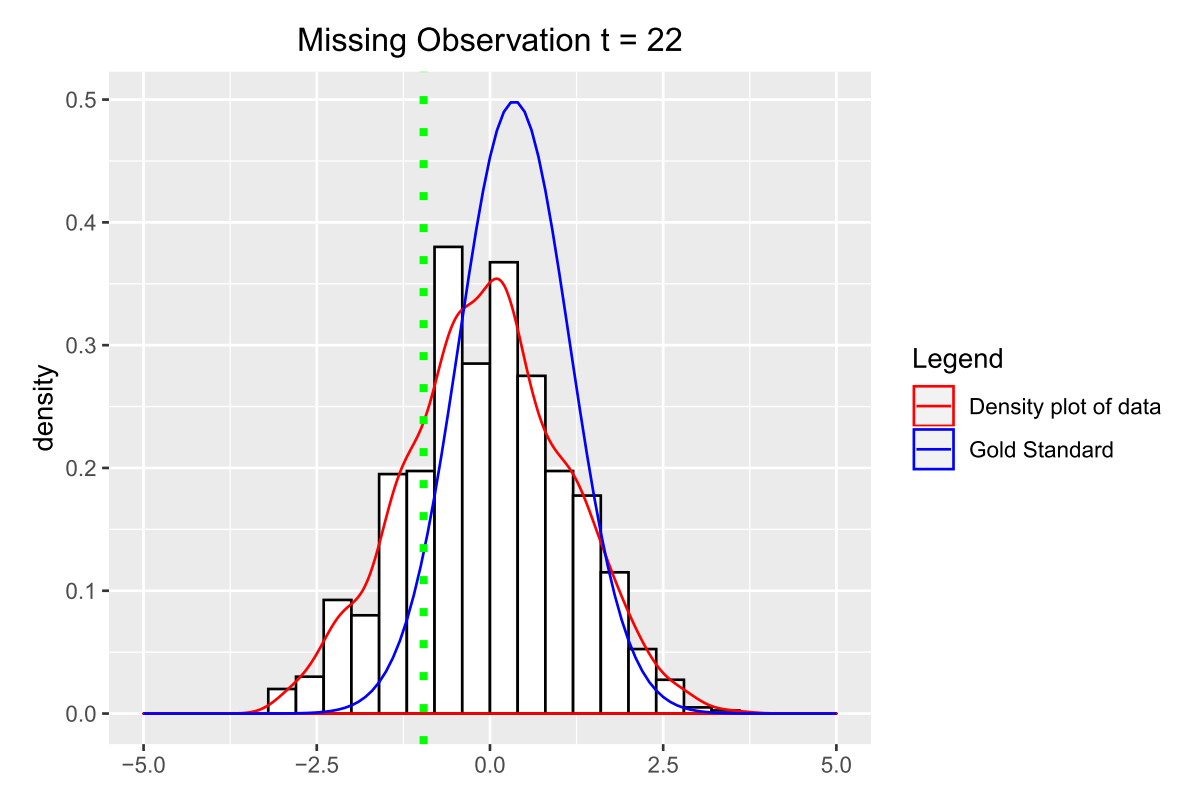
\includegraphics[width=0.5\linewidth]{ar1_001.PNG}}
    \subfloat[fig 2]{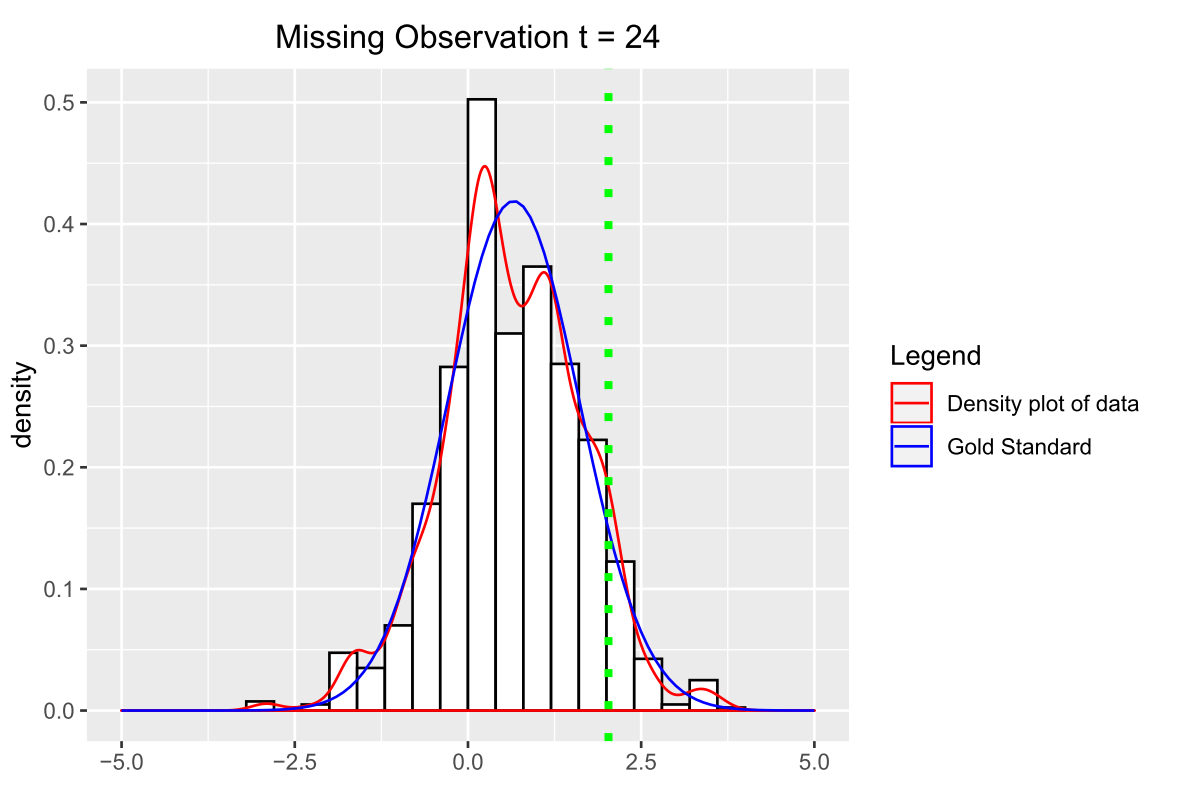
\includegraphics[width=0.5\linewidth]{ar1_002.PNG}}\\
    \subfloat[fig 3]{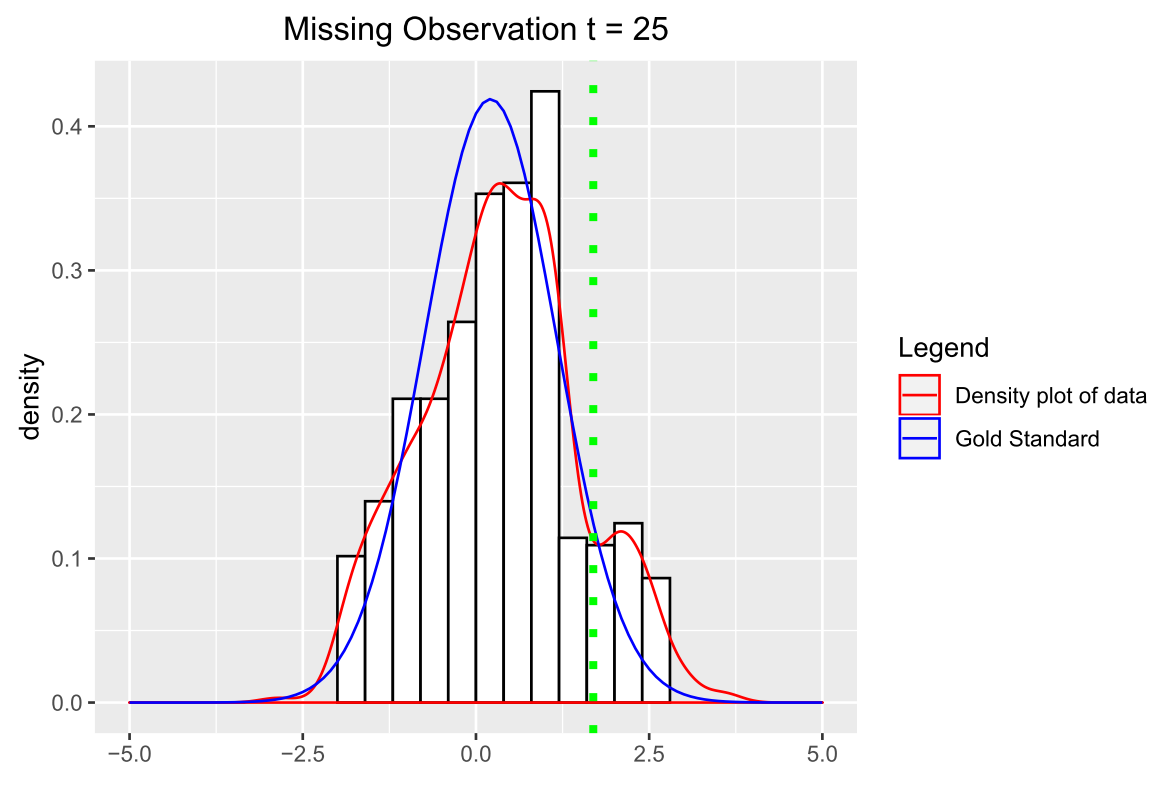
\includegraphics[width=0.5\linewidth]{ar1_003.PNG}}
    \subfloat[fig 4]{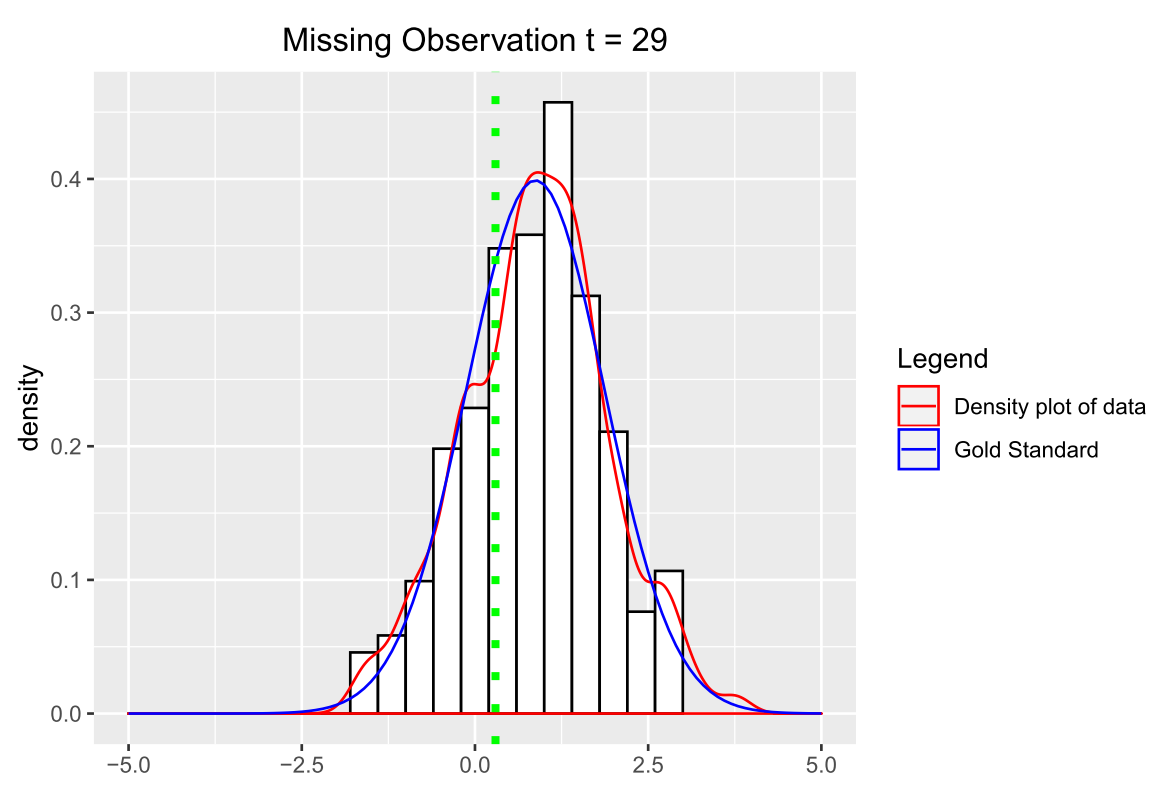
\includegraphics[width=0.5\linewidth]{ar1_004.PNG}}\\
    \subfloat[fig 5]{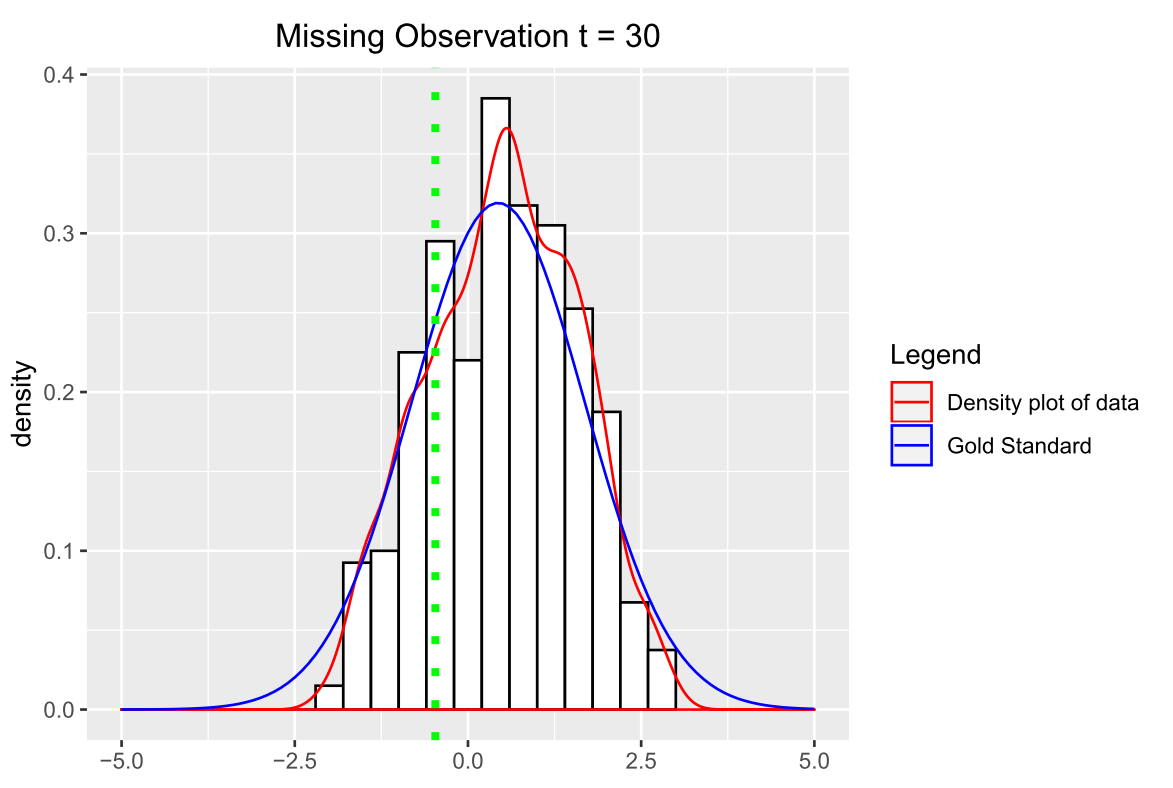
\includegraphics[width=0.5\linewidth]{ar1_005.PNG}}
    \caption{AR(1) MODEL: Simulations with 1,000 particles and 30 times compared to the gold standard for the 5 missing times of the AR(1) model. In Green the value for the observation. The AR(1) model had parameter $\varphi = 0.5$, variance $\sigma^2 = 1$. The Bernoulli distribution had parameter $p = 0.2$}
\label{fig:1}
\end{figure*}

\begin{figure*}
    \includegraphics[width=\textwidth]{river_007.png}
    \caption{RIVER INVASION: Simulations with 1,000 particles and 50 cells of 3 possible river invasions all with probability of invasion $\theta = 0.3$ but with different values of the parameter $\varphi$ for the probability of the observations. Figures A1, B1 and C1 show the simulations of the 3 invasions while figures A2, B2 and C2 show the same simulations but with the observations superimposed in red. A1 and A2 show the invasion with $\varphi = 0.3$, B1 and B2 show the invasion with $\varphi = 0.1$. Figure C1 and C2 show the invasion with $\varphi = 0.8$.}
    \label{fig:2}
\end{figure*}

\section{Conclusions and further developments}
\label{sec:9}

{\color{blue} The present investigation shows how our new methodology can be used to estimate the past and present state of a system for which incomplete information is continuously gathered. In particular in the case of invasive species it will be well suited to estimate the past trajectories and current extent of an invasion. This could be then used to help understanding the efficacy of an eradication program or to inform on where to search for currently hidden invades or to assess the risk from currently unobserved individuals.

As mentioned in the introduction, different methods exist to numerically solve estimations problems with exact but incomplete observations in an online manner. However, our method is the first one, at the best of our knowledge, that uses corrections seeking to improve previous estimations as each new observation is acquired. VVV Jon, I think this sentence is really important, is there anything I should/could add to show how innovative or different the method is?}

The methodology could also be used in the more complex scenario where not only we have entire cases unobserved, but also the number of missing cases is unknown, {\color{blue} for example, in more general predictive modeling of a species geographical distribution.}

In this context we are planning to apply our new method to a specific invasive species problem: the fire ants invasion in Queensland, Australia. This application will seek to improve and complement the existing agent based approach developed by Keith and Spring (\cite{Keith}). {\color{blue} Their method consisted of constructing a likelihood model in terms of some unknown parameters that included, among other things, the phylogeny, jump type, founding type and treatment success rate. The posterior distribution was then sampled using a generalised Gibbs technique that enabled transdimensional sampling, which is used when the number of parameters is unknown, as in their case. However, their method needed to be re-run each time new data was available and could not be updated online.}

The results we have for the AR(1) model compared to the gold standard show that our simulations closely approximate analytical solutions, while the rive example shows the applicability of the method to a simple invasive species problem.

Our algorithm is also reasonably fast as the weights involve cancellations that significantly reduce the calculations required. However, we might need to optimise and further maximise efficiency when running with bigger data sets. For example, we could apply a more efficient resampling step.

We are planning to adapt the methodology to be applied to time continuous models, and we also envisage the possibility of improving our approach to allow for non-deterministic revision of imputed values that, while not inconsistent with later observations, can nevertheless be updated in light of new information. This will require a different definition of the probability $p^*$ and some more theoretical proof of its existence and validity. 

%\begin{acknowledgements}
%If you'd like to thank anyone, place your comments here
%and remove the percent signs.
%\end{acknowledgements}

\begin{thebibliography}{}

\bibitem [\protect\citeauthoryear{Beer}{1990}]{Beer} 
Beer, T.: The Australian National Bushfire model project. Math Comput. Model. 13(12), 49-56 (1990).

\bibitem [\protect\citeauthoryear{Capp\'{e} et al.}{2005}]{Cappe} 
Capp\'{e}, O., Moulines, E., Ryd\'{e}n, T.: Inference in Hidden Markov Models. Springer Series in Statistics. Springer (2005).

\bibitem [\protect\citeauthoryear{Del Moral et al.}{2015}]{Del Moral} 
Del Moral, P., Murraly, L.M.: Sequential Monte Carlo with Highly Informative Observations. SIAM/ASA Journal on Uncertainty Quantification 3(1), 969-997 (2015).

\bibitem [\protect\citeauthoryear{Doucet and Johansen}{2011}]{Doucet} 
Doucet, A., Johansen, A.M.: A tutorial on particle filtering and smoothing: Fifteen years later. In Crisan, D. and Rozovskii, B., editors, The Oxford Handbook of Nonlinear Filtering, Oxford Handbooks, chapter 24, pages 656–704. Oxford University Press. (2011).

\bibitem [\protect\citeauthoryear{Finke et al.}{2019}]{Finke} 
Finke, A., King, R., Beskos, A., Dellaportas P.: Efficient Sequential Monte Carlo Algorithms for Integrated Population Models. JABES 24, 204–224 (2019).

\bibitem [\protect\citeauthoryear{Keith and Spring}{2013}]{Keith} Keith, J. M., Spring, D.: Agent-based Bayesian approach to monitoring the progress of invasive species eradication programs. Proc Natl Acad Sci, 110(33): 13428-13433 (2013).

\bibitem [\protect\citeauthoryear{Kong et al.}{1994}]{Kong} Kong, A., Liu, J.S., Wong, W.H.: Sequential Imputations and Bayesian Missing Data Problems. Journal of the American Statistical Association, 89(425): 278-288 (1994).

\bibitem [\protect\citeauthoryear{Little and Rubin}{2019}]{Little} Little, R, Rubin, D.: Statistical Analysis with Missing Data, Third Edition. Wiley, New York (2019).

\bibitem [\protect\citeauthoryear{Malathy and Baboo}{2011}]{Malathy} 
Malathy, A., Baboo, S.S.: An Enhanced Algorithm to Predict a Future Crime using Data Mining. Int. J. Comput. Appl. 21(1), 1-6 (2011).

\bibitem [\protect\citeauthoryear{Nakagawa}{2015}]{Nakagawa}
Nakagawa, S.: Missing data. In: Fox G.A., Negrete-Yankelevich S., Sosa V.J. (eds.) Ecological Statistics: Contemporary theory and application, pp 81-105. Oxford University Press (2015). 

\bibitem[\protect\citeauthoryear{O'Neill and Robers}{2002}]{O'Neill}
O'Neill, P.D., Roberts G.O.: Bayesian inference for partially observed stochastic epidemics. J. R. Stat. Soc. A. Stat. 162(1), 121-129 (2002).

\bibitem[\protect\citeauthoryear{Rohlin}{1962}]{Rohlin}
Rohlin V.A.: On the fundamental ideas of measure theory.  Trans.
Amer. Math. Soc. 1(10), 1-52 (1962).

\bibitem [\protect\citeauthoryear{Rubin}{1987}]{RubinMI}
Rubin, D.B.: Multiple imputation for nonresponse in surveys. Wiley, New York (1987).

\bibitem [\protect\citeauthoryear{Tanner and Wong}{1987}]{Tanner}
Tanner, M.A., Wong, W.H.: The Calculation of Posterior Distributions by Data Augmentation. J. Am. Stat. Assoc. 82(398), 528-540 (1987).

\bibitem [\protect\citeauthoryear{Young}{2011}]{Young}
Young, P.C.: Recursive Estimation and Time-Series Analysis. Springer-Verlag Berlin Heidelberg (2011).

\bibitem [\protect\citeauthoryear{Zhang et al.}{2015}]{Zhang}
Zhang, X., Khwaja A. S., Luo J., Housfater A.S., Anpalagan A.: Multiple Imputations Particle Filters: Convergence and Performance Analyses for Nonlinear State Estimation with Missing Data. IEEE J. Sel. Top Signa. 9(8), 1536-1547 (2015).

\end{thebibliography}


\clearpage
\appendix

\begin{algorithm}[H]
\caption{SIR with corrections for an AR(1) model}\label{euclid}
 \begin{algorithmic}

 \State  \bf{Initialize:} \normalfont At time t = 1
            
\begin{enumerate}
	\item For $i = 1, \dots , n$
	\begin{enumerate}
		\item Sample $(x_{1})_i \sim \mathcal{N} \Bigg (0, \frac{\sigma^2}{1- \varphi^2} \Bigg)$ and $(b_1)_i \sim Bernoulli(\theta)$
		\item Evaluate the importance weights up to a normalising constant:
		\[
		\tilde{w}^{1}_{i} = 1
		\]
	\end{enumerate}
	\item For $i = 1, \dots , n$ normalise the importance weights: 
	\[
	w^{1}_{i} = \frac{1}{n}
	\]
\end{enumerate}

 \State  \bf{Iterate:} \normalfont For $t$ from 2 to $N$

\begin{enumerate}
	\item For $i = 1, \dots , n$
	\begin{enumerate}
  		\item sample $(x_t)_i \sim \mathcal{N} (\varphi (x_{t-1})_i, \sigma^{2})$ and $b^t_{i} \sim Bernoulli(\theta)$.
		\item {Correct every element of $\vec{x}^t_i$ in light of the data $\vec{z}^t$ to obtain new samples $(\vec{x'})^t_i$ directly substituting the new data: for $s = 1, \dots ,t$ if $(z^t)_s \neq -$, $((x')_i^t)_s = (z^t)_s$ else if $(z^t)_s = -$, $((x')_i^t)_s = (x^t_i)_s$.}
		\item Correct every element of $\vec{b}_i^t$ in light of the data $\vec{z}^t$ to obtain new samples $(\vec{b'})^t_i$ substituting 0s when $(z^t)_s = -$ and 1s otherwise for $s = 1, \dots, t$.
		\item Evaluate the weights up to a normalising constant using equation (\ref{eq:2}):
		\[
		\tilde{w}^{t}_{i} = \frac{q(\vec{(x')}^{t}_i, \vec{(B')}^{t}_i | \vec{Z}^{t-1})}{q(\vec{x}^{t}_i, \vec{B}^{t}_i | \vec{Z}^{t-1})}
		\]
	\end{enumerate}
	\item For $i = 1, \dots , n$ normalise the importance weights:
	\[
	w^{t}_{i} = \frac{\tilde{w}^t_i}{\sum_{k=1}^{n}\tilde{w}^{t}_k}
	\]
	\item Perform resampling
	\begin{enumerate}
	    \item Draw $n$ particles from the current particle set with probabilities proportional to their weights. Replace the current particle set with the new $n$ particles.
	    \item Set $w^t_i=1/n$
	\end{enumerate}
\end{enumerate}
  
 \end{algorithmic}
\end{algorithm}

\begin{algorithm}[H]
\caption{SIR with corrections for an river invasion}\label{euclid}
 \begin{algorithmic}

 \State  \bf{Initialize:} \normalfont At time t = 1
            
\begin{enumerate}
	\item For $i = 1, \dots , n$
	\begin{enumerate}
	    \item For $s = 1, \dots, N$
		First observation $z_m$ known: For each particle, at time 1, fill the invasion vector of $\vec{x}_i^t$ size N with $(x_{m})^1_i = 1$ and $(x_{s})^1_i = 0$ if $s \neq m$. 
		For each particle, at time 1, fill the invasion vector $\vec{z}_i^t$ of size N with $(z_m)^1_i = 1$ and $(z_{s})^1_i = 0$ if $s \neq m$.
		\item Evaluate the importance weights up to a normalising constant:
		\[
		\tilde{w}^{1}_{i} = 1
		\]
	\end{enumerate}
	\item For $i = 1, \dots , n$ normalise the importance weights: 
	\[
	w^{1}_{i} = \frac{1}{n}
	\]
\end{enumerate}

 \State  \bf{Iterate:} \normalfont For $t$ from 2 to $T$

\begin{enumerate}
	\item For $i = 1, \dots , n$
	\begin{enumerate}
  		\item Sample $(r)^t_i \sim Bernoulli(\theta)$ and $(l)^t_i \sim Bernoulli(\theta)$. For $s = 1, \dots, N$ for each particle, at time t, fill the invasion vector $\vec{x}_i^t$ of size N with the values of $\vec{x}_i^{t-1}$ then substitute $(x_s)^t_i = (r)^t_i$ for $s$ s.t. $(x_{s-1})^{t-1}_i = 1$ and $(x_s)^{t-1}_i = 0$ and substitute $(x_s)^t_i = (l)^t_i$ for $s$ s.t. $(x_s)^{t-1}_i = 0$ and $(x_{s+1})^{t-1}_i = 1$.
  		\item Sample k elements $(a_k)^t_i \sim Bernoulli(\varphi)$ until the first 0 is sampled, and h elements $(b_h)^t_i \sim Bernoulli(\varphi)$ until the first 0 is sampled. For $s = 1, \dots, N$ for each particle, at time t, fill the observation vector $\vec{z}_i^t$ of size N with the values of $\vec{z}_i^{t-1}$ then substitute the k elements $(z_{s+k})^t_i = (r)^t_i$ for $s$ s.t. $(z_{s-1})^{t-1}_i = 1$ and $(z_s)^{t-1}_i = 0$ and substitute the h elements $(z_{s-h})^t_i = (l)^t_i$ for $s$ s.t. $(z_s)^{t-1}_i = 0$ and $(z_{s+1})^{t-1}_i = 1$.
		\item Correct every element of $\vec{x}^t_i$ in light of the data $\vec{z}^t$ to obtain new samples $(\vec{x'})^t_i$ directly substituting the new data: for $s = 1, \dots ,N$ if $(z^t)_s = 1$, $((x')_i^t)_s = 1$ else if $(z^t)_s = 0$, $((x')_i^t)_s = (x^t_i)_s$. Correct every element of $\vec{z}^t_i$ in light of the data $\vec{z}^t$ to obtain $(\vec{z'})^t_i$ simply substituting $(\vec{z'})^t_i$ with $\vec{z}^t$.
		\item Evaluate the weights up to a normalising constant using the values for $q$ from equation (\ref{eq:4}):
		\[
		\tilde{w}^{t}_{i} = \frac{q(\vec{(X')}^{t}_i, \vec{(z')}^{t}_i | \vec{Z}^{t-1})}{q(\vec{X}^{t}_i, \vec{z}^{t}_i | \vec{Z}^{t-1})}
		\]
	\end{enumerate}
	\item For $i = 1, \dots , n$ normalise the importance weights:
	\[
	w^{t}_{i} = \frac{\tilde{w}^t_i}{\sum_{k=1}^{n}\tilde{w}^{t}_k}
	\]
	\item Perform resampling
	\begin{enumerate}
	    \item Draw $n$ particles from the current particle set with probabilities proportional to their weights. Replace the current particle set with the new $n$ particles.
	    \item Set $w^t_i=1/n$
	\end{enumerate}
\end{enumerate}
  
 \end{algorithmic}
\end{algorithm}

\end{document}

